\chapter{AFIDs-Data: MRI datasets with anatomical fiducial annotations}\label{chap:afidsdata}
\newpage
\sloppy
\noindent This chapter is largely based on:
\begin{itemize}[noitemsep,topsep=0pt]
    \begin{small}
    \item
    A. Taha, G. Gilmore, M. Abbass, J. Kai, T. Kuehn, J. Demarco, G. Gupta, C. Zajner, D. Cao, R. Chevalier, A. Ahmed, A. Hadi, B.G. Karat, O.W. Stanley, P.J. Park, K.M. Ferko, D. Hemachandra, R. Vassallo, M. Jach, A. Thurairajah, S. Wong, M.C. Tenorio, F. Ogunsanya, A.R. Khan, J.C. Lau.
    \end{small} Magnetic resonance imaging datasets with anatomical fiducials for quality control and registration. \textit{Scientific Data}, 10:449, 2023.
    
\end{itemize}

\section{Background and Summary}
Open resources available for reproducible, quantitative assessment of brain correspondence have been limited. The most common metrics employed for the purpose of examining the quality of image registration, including the Jaccard similarity and Dice kappa coefficients, compute the voxel overlap between regions of interest (ROIs), which have been shown to be insufficiently sensitive when used in isolation or in combination for validating image registration strategies \cite{Rohlfing2012-kt}. The ROIs used in voxel overlap are often larger subcortical structures that are readily visible on magnetic resonance imaging (MRI) scans (e.g., the thalamus, globus pallidus, and striatum), and thus lack the ability to detect subtle misregistration between images which may be crucial where millimetric differences in variability should be accounted for \cite{Rohlfing2012-kt,Lau2019-eh,Abbass2022-lf,Chakravarty2009-kq}.

Inspired by classic stereotactic methods, our group created, curated, and validated a protocol for the placement of anatomical fiducials (AFIDs) on structural MRI scans of the human brain \cite{Lau2019-eh}. The protocol involves the placement of 32 AFIDs found to have salient features that allow for accurate localization. The AFIDs are described using three-dimensional (x, y, and z) Cartesian coordinates and thus correspondence between points can be computed using Euclidean distances across a variety of applications. After a brief tutorial, AFIDs have been shown to be highly reproducible even when performed by individuals with no prior knowledge of medical images, neuroanatomy, or neuroimaging software. This was shown in separate studies where placements were performed on publicly available templates and datasets \cite{Lau2019-eh} and a clinical neuroimaging dataset \cite{Abbass2022-lf}.

The AFID protocol provides a metric that is independent of the registration itself while offering sensitivity to registration errors at the scale of millimeters (mm). This margin is crucial in neuroimaging applications (including morphometric analysis and surgical neuromodulation), where a few millimeters may represent the difference between optimal and suboptimal therapy.

The aim of this data descriptor is to provide the community with curated AFID placements and their associated MRI images. We release annotations on five datasets (\(N\)=202; 6,464 fiducials) including healthy subjects and patients with neurological disorders, and 14 commonly used MRI templates (4,288 fiducials), totalling 300 human rater hours of manual annotations. Descriptions of the datasets and templates are provided in subsequent sections. We highlight current and prospective applications of our released data in Figure \ref{fig:ch2_Figure_1}.

\begin{figure}[hbt!]
    \centering
    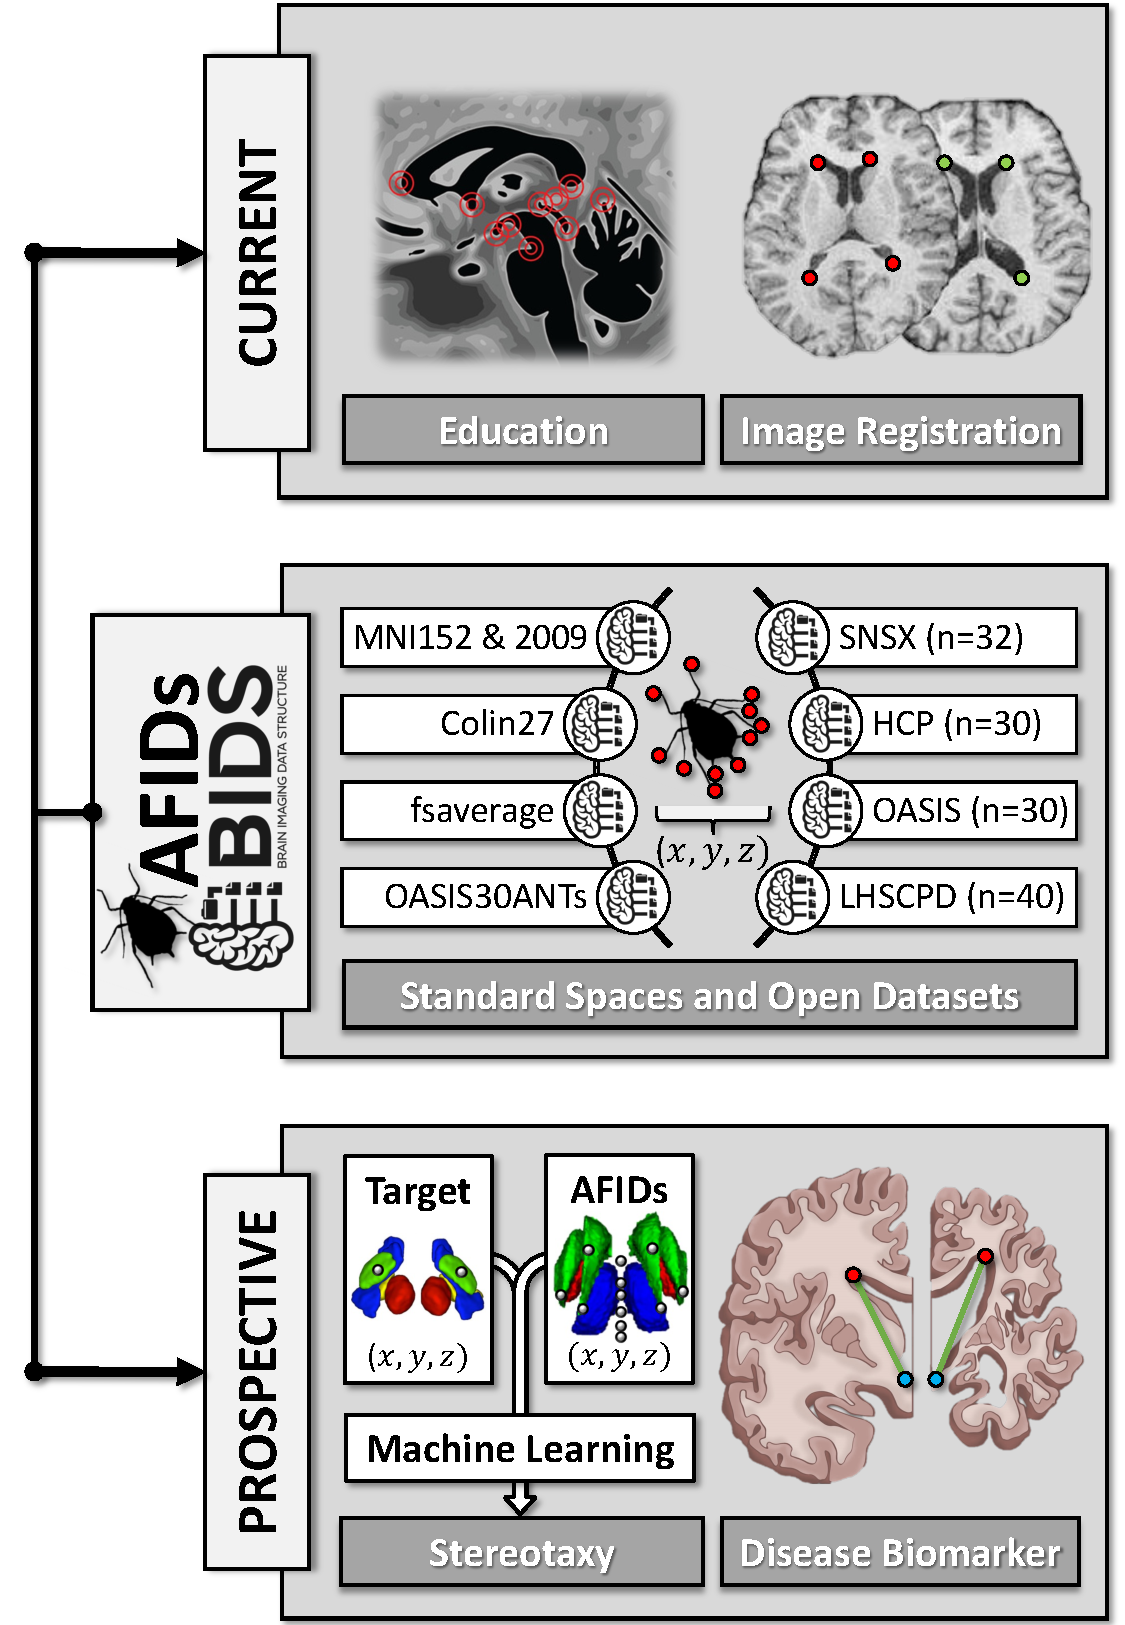
\includegraphics[width=0.85\linewidth]{figs/ch2_Figure_1.pdf}
    \caption{Current and prospective applications of curated anatomical fiducial (AFID) placements. Top Panel: Current applications in neuroanatomy education and image registration. Middle Panel: Released healthy and pathologic datasets and templates (detailed descriptions can be found in text). Bottom Panel: Prospective applications of AFIDs in stereotactic targeting and as a disease biomarker.}
    \label{fig:ch2_Figure_1}
\end{figure}


\section{Current Applications}
\subsection{Registration Assessment}
We share our curated AFID annotations for a wide variety of datasets and templates of varying field strengths. This diversity of datasets will facilitate the testing and validation of image registration algorithms that can be used in many contexts. The user can select the datasets and templates that are in line with their neuroimaging application, then use the curated annotations to assess image registration quantitatively. For instance, AFIDs have been used to evaluate the process of iterative deformable template creation \cite{Xiao2019-ao,Lau2020-dh} showing that error metrics generated from AFIDs converged differently as a function of template iterations and registration method (i.e., linear vs non-linear). Sharing the AFID placements and their associated images in the Brain Imaging Data Structure (BIDS) format aids in the convenience we strive to provide for the end-user and neuroimaging application developer.

\subsection{Education}
New raters can learn to view and localize anatomical regions using our AFID framework then autonomously compare their placements to the curated normative distribution placements we release here. Our placements have been compiled over the years and can help raters assess accuracy for specific fiducials across subjects and template data. To improve user accessibility and navigation of our released AFID annotations and framework, we also release the AFIDs validator (\url{https://validator.afids.io}; see Figure \ref{fig:ch2_Figure_2}). This tool provides: (1) detailed descriptive and visual documentation of the AFID placement protocol, (2) an interactive way for users to upload placements to a regulated database, and (3) interactive methods to view uploaded placements relative to curated placements almost instantaneously, which helps guide users to improve neuroanatomical understanding and placement accuracy.

\subsection{Brain Structure and Volumetric Analyses}
AFIDs and their associated images in our pathological dataset, when compared to those from healthy controls, offer a valuable framework for investigating structural brain differences. This comparison can reveal subtle morphological changes associated with disease, support the identification of putative biomarkers for neurodegenerative conditions, and contribute to the development of normative brain models that account for pathological variation.

\begin{figure}
    \centering
    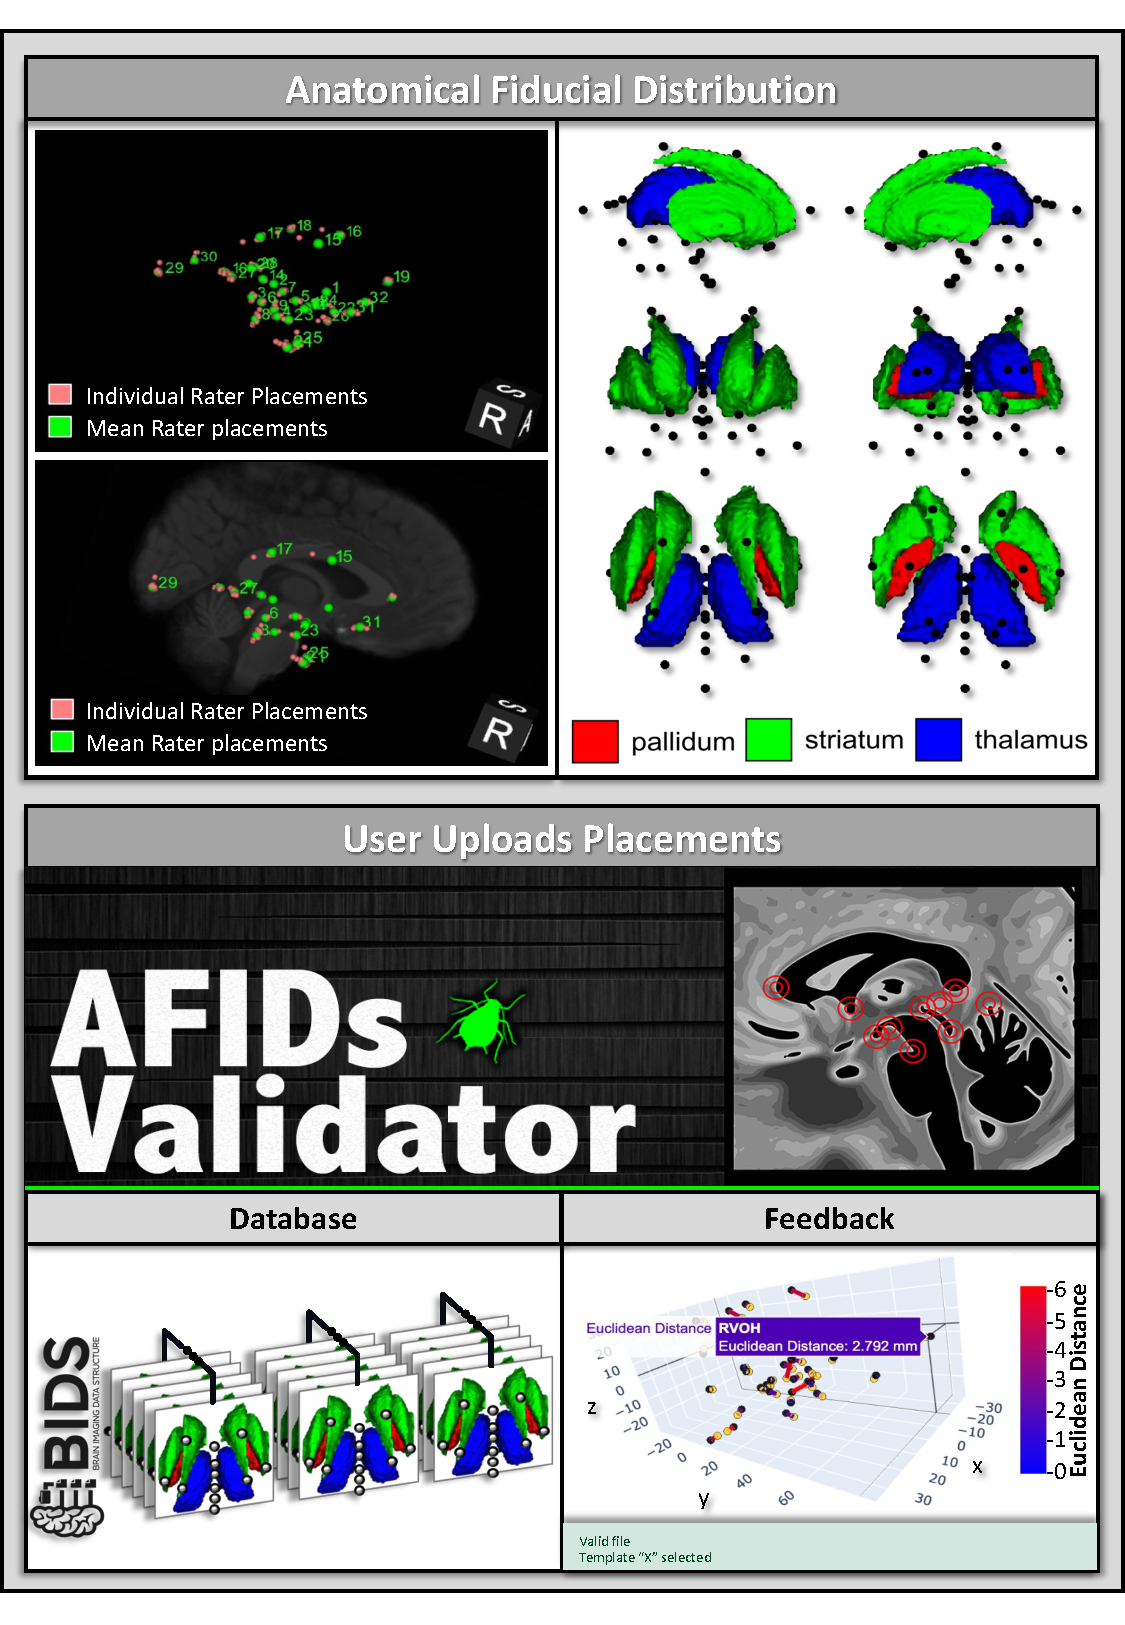
\includegraphics[width=0.9\linewidth]{figs/ch2_Figure_2.pdf}
    \caption{Curated AFID locations within the brain and usage of the AFIDs validator website. Top Panel: Distribution of AFIDs overlayed on one of the released templates. We also show major subcortical structures with AFIDs (black points) in various anatomical views. Bottom Panel: Uses and outputs from the AFIDs validator website \url{https://validator.afids.io}. The user decides whether to upload their placements to our database and will receive summary metrics regarding their placements in an interactive 3D coordinate system and tabular format (not shown).}
    \label{fig:ch2_Figure_2}
\end{figure}

\section{Prospective Applications}
\subsection{Registration Optimization and Quality Control}
The released imaging and AFID placement data is useful in a few ways for improving neuroimaging pipelines: (1) providing centralized and quality controlled neuroimaging data (from 4 different neuroimaging datasets) allowing for a more accurate and generalizable head-to-head comparison among existing software for image registration, and (2) establishing a new registration metric that can be incorporated into neuroimaging software development workflows to optimize registration algorithm performance and ensure quality control.

\subsection{Automatic and Accurate Landmark Placement}
Our curated AFIDs can serve as ground truth placements when training machine learning algorithms to automate brain landmark localization. Among the 32 AFIDs we release are the anterior and posterior commissures (AC and PC, respectively). Downstream applications of automatic localization include automatically computing AC-PC transformation (a common process in neuroimaging studies) and aspects of neurosurgical planning that involve the placement of these anatomical landmarks. The diversity of the released data (both hardware and disease status) will be crucial to the generalizability of such tools.

\subsection{Surgical Targeting}
We release locally curated ultra-high field (7-Tesla; 7-T) MRI data where small structures like the subthalamic nucleus (STN) and zona incerta within the posterior subthalamic area are clearly visible \cite{Keuken2013-ax, Lau2020-dh}. Ground truth locations of surgical targets (x, y, and z) can be related to AFID locations via predictive models. This approach mitigates the lack of access to best-case neuroimaging in clinical settings due to limited access to high-field MRI or motion degradation.

\subsection{Brain Anatomy Abstraction and Anonymization}
AFIDs and the distances between them represent an abstraction of brain anatomy in an anonymized way while still allowing for the accurate pooling of data. Other significant anatomical landmarks (representing lesions, tumors, or other structures) can be described in reference to the AFID “coordinate system” we establish using these curated placements.

\section{Methods}
\subsection{Fiducial Selection and Placement Assessments}
The current version of the AFID protocol involves the placement of 32 landmarks. They were selected to be easily identified on structural MRI scans across varying field strengths (1.5T, 3T, 7T). During the selection process, regions that were prone to geometric inhomogeneity and distortion were avoided to enhance the accuracy of fiducial placement. There are 10 fiducials that fall on the midline and 11 located laterally on both hemispheres (see Table 1). The AFID protocol includes landmarks representing salient neuroanatomical features mostly located in the subcortex (see Figure \ref{fig:ch2_Figure_2}).

\begin{table}[ht]
\caption{List of anatomical fiducials (AFIDs), their acronyms, and laterality. Fiducials with paired left/right locations are grouped together.}
\centering
\begin{tabular}{cccc}
\toprule
\textbf{Number} & \textbf{Anatomical Fiducial} & \textbf{Acronym} & \textbf{Side} \\
\midrule
1         & Anterior commissure                      & AC          & Midline \\
2         & Posterior commissure                     & PC          & Midline \\
3         & Infracollicular sulcus                   & ICS         & Midline \\
4         & Pontomesencephalic junction              & PMJ         & Midline \\
5         & Superior interpeduncular fossa           & SIPF        & Midline \\
6, 7      & Superior lateral mesencephalic sulcus    & R/L SLMS    & Lateral \\
8, 9      & Inferior lateral mesencephalic sulcus    & R/L ILMS    & Lateral \\
10        & Culmen                                   & CUL         & Midline \\
11        & Intermammillary sulcus                   & IMS         & Midline \\
12, 13    & Mammillary body                          & R/L MB      & Lateral \\
14        & Pineal gland                             & PG          & Midline \\
15, 16    & Lat. aspect frontal horn at AC           & R/L LVAC    & Lateral \\
17, 18    & Lat. aspect frontal horn at PC           & R/L LVPC    & Lateral \\
19        & Genu of corpus callosum                  & GENU        & Midline \\
20        & Splenium of corpus callosum              & SPLE        & Midline \\
21, 22    & Anterolateral temporal horn              & R/L ALTH    & Lateral \\
23, 24    & Sup. anteromedial temporal horn          & R/L SAMTH   & Lateral \\
25, 26    & Inf. anteromedial temporal horn          & R/L IAMTH   & Lateral \\
27, 28    & Indusium griseum origin                  & R/L IGO     & Lateral \\
29, 30    & Ventral occipital horn                   & R/L VOH     & Lateral \\
31, 32    & Olfactory sulcal fundus                  & R/L OSF     & Lateral \\
\bottomrule
\end{tabular}
\label{tab:afid_list}
\end{table}
\newpage
Fiducial localization error (FLE) is a term described by Fitzpatrick and colleagues \cite{Fitzpatrick1998-hp} that represents the distance between a fiducial position and its intended location. This term is commonly used when operating image-guidance systems during surgical procedures. In the context of the AFID protocol, and inspired by this extant terminology, we define the term \textbf{anatomical fiducial localization error (AFLE)}. This value, measured in millimeters, reflects the error arising from the placement (i.e., localization) of each fiducial. When used to communicate the accuracy of all AFIDs together, we refer to this as the \emph{global AFLE}. There are three contexts for applying AFLEs (Figure \ref{fig:ch2_Figure_AFLE}):
\begin{enumerate}
    \item \textbf{Mean AFLE:} Rater localization error relative to the intended location, defined as the mean placement of all raters for a specific fiducial (termed the \emph{ground truth AFID} in subsequent sections).
    \item \textbf{Inter-rater AFLE:} Rater localization error calculated as the pairwise distances between different rater placements. If a single rater performed the AFID protocol more than once, their mean placement coordinates were used for pairwise distance calculations.
    \item \textbf{Intra-rater AFLE:} Rater localization error evaluating the precision of multiple placements by a single rater, computed as the average pairwise distance between that rater’s placements.
\end{enumerate}

\begin{figure}[hbt!]
    \centering
    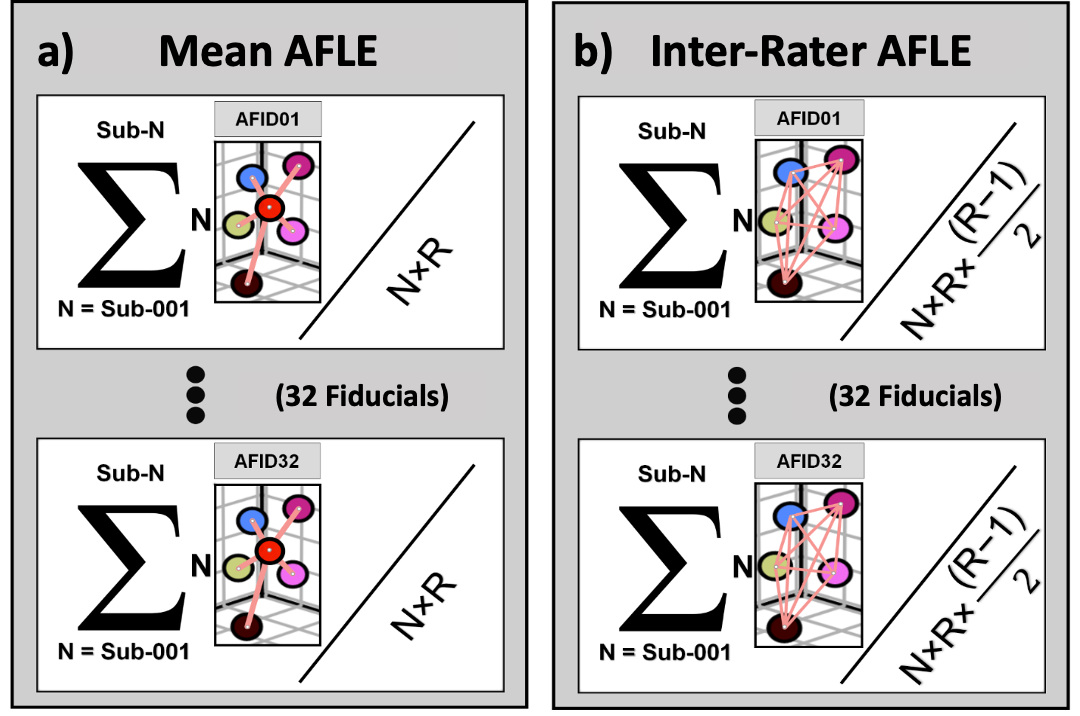
\includegraphics[width=1\linewidth]{figs/ch2_Figure_AFLE.png}
    \caption{
    Technical validation computations for anatomical fiducial (AFID) placements across templates and datasets. (a) and (b) display the equations used to compute mean and inter-rater anatomical fiducial localization error (AFLE), respectively. $N$ denotes the number of subjects in a dataset. For templates, $N = 1$. $R$ represents the number of raters per scan/image. In (a), Euclidean distances (shown in pink) are measured from each rater placement to the ground-truth fiducial (shown in red). The mean AFLE is computed by summing all such distances across subjects and dividing by the total number of distances per AFID ($N \times R$). In (b), Euclidean distances (pink) represent all pairwise distances between rater placements for a given scan. Inter-rater AFLE is computed by summing all pairwise distances and dividing by the total number of pairwise combinations per AFID across the dataset, given by $N \times R \times \frac{(R - 1)}{2}$.
    }    
\label{fig:ch2_Figure_AFLE}
\end{figure}

We also adopt the term \textbf{fiducial registration error (FRE)} in the context of the AFID protocol, and refer to it as the \textbf{anatomical fiducial registration error (AFRE)}. It is important to note that AFRE in our context diverges from the original usage by Fitzpatrick and colleagues\cite{Fitzpatrick1998-hp}, which was restricted to describing registration error at fiducials used to drive image registration (i.e., during landmark-based registration). Computed in millimeters, AFRE is defined as the error arising from the registration protocol performed between two images (often, but not limited to, subject and template). AFRE is the distance, after co-registration, between each of the 32 AFIDs placed on a moving image and their counterparts placed on the fixed image (i.e., homologous points). Thus, the AFRE provides a registration error metric that is independent of the registration protocol. The average AFRE of all fiducials is termed the \emph{global AFRE}. We  establish nomenclature to differentiate use cases for AFRE:
\begin{itemize}
    \item \textbf{Real-world AFRE:} If an individual rater placement is chosen for subsequent analysis, the resulting AFRE is referred to as the real-world AFRE, as it reflects what would occur in a clinical setting where one rater applies the AFID protocol.
    \item \textbf{Consensus AFRE:} If a ground truth AFID placement is used, the resulting error is termed the consensus AFRE, as it represents the average placement among a group of raters prior to the image registration step.
\end{itemize}

\subsection{Hardware and Software}
All manually curated AFIDs were placed using the Markups Module of 3DSlicer \cite{Fedorov2012-rk}, which is a commonly used open-source imaging software. The datasets were curated at different times so a reference to the exact version of 3DSlicer and associated modules will be made under each dataset. 3DSlicer was chosen because it offers a variety of modules, particularly markups and registration modules used for fiducial placement and AC-PC transformation. 3DSlicer stores points placed within its 3D coordinate system overlaid on the image giving the possibility of more accurate localization without the need to interpolate to the nearest voxel. The AFID placements released here for templates and datasets were performed on structural T1w MRI images.

\subsection{Performing the AFID Protocol}
All raters underwent extensive training before being involved in any AFID related studies. More specifically, they (1) attended a synchronous session about 3DSlicer and placed all the AFIDs under the supervision of expert raters, (2) were asked to refer to resources found on our AFID protocol website \url{https://afids.github.io/afids-protocol} to supplement their learning asynchronously, and (3) uploaded their annotations to the AFIDs validator tool for feedback with further review with an expert to ensure that their annotations were of sufficient quality. We collected demographic data (neuroanatomy, imaging, and 3DSlicer exposure) for raters involved in data curation (see Data Records).
For manual rater placements, the AFID protocol generally began with the placement of the anterior commissure (AC) and posterior commissure (PC) points (AFID01 and 02, respectively), which are defined to be at the center of each commissure. This was then followed by the identification of one or two more midline points (often the pontomesencephalic junction, AFID04, and the genu of corpus callosum, AFID19, are used). After that, an AC-PC transformation is performed, and the rest of the anatomical fiducials are placed. Rater placements deviating from a ground truth fiducial by greater than 10 mm were removed and considered outliers, as these errors are likely to be due to mislabelling and not reflective of true localization accuracy. In addition to subsequent sections, Table \ref{tab:afid_datasets} provides brief descriptions of the released datasets and templates, information about raters, and AFID placements.

\begin{sidewaystable}
\centering
\caption{Summary of datasets and templates annotated with anatomical fiducials (AFIDs), including acquisition field strength, number of raters, and total number of annotations. Some datasets are primarily image templates; others include subject-level data.}
\begin{tabular}{
  >{\centering\arraybackslash}m{3cm}
  >{\centering\arraybackslash}m{9cm}
  >{\centering\arraybackslash}m{1.5cm}
  >{\centering\arraybackslash}m{3.5cm}
  >{\centering\arraybackslash}m{3cm}
}
\toprule
\textbf{Dataset} & \textbf{Description} & \textbf{Scanner} & \textbf{Raters (N)} & \textbf{Imaging} \\
\midrule
MNI2009bAsym & A population template (N=152) commonly used in the neuroimaging literature  & 1.5 & 8 novices & \cite{Fonov2009-oi} \\[2pt]

MNIColin27 & Single subject average (N=27) & 1.5 & 8 novices & \cite{Holmes1998-mb} \\[2pt]

Agile12v2016 & UHF template (N = 12) created at Western University & 7 & 8 novices & \cite{Lau2018-fp} \\[2pt]

BigBrainSym & Ultra-high-res histological brain (BigBrain) registered to MNI2009bSym & N/A & 2 experts & \cite{Amunts2013-vu}, \cite{Xiao2019-ao} \\[2pt]

MNI2009bSym & Symmetric version of MNI2009bAsym & 1.5 & 2 experts & \cite{Fonov2009-oi} \\[2pt]

PD-25 & Multi-contrast MNI template of a Parkinson’s disease cohort & 3 & 2 experts & \cite{Xiao2017-zp} \\[2pt]

TemplateFlow & A centralized resource of open-access templates for neuroimaging studies (tpl-MNI152 -Lin, NLin2009cAsym, NLin2009cSym, NLin6Asym, NLin6Sym, tpl-MNI305, tpl-OASIS30ANTs, tpl-fsaverage) & 3+ & 1 expert, 3 novices & \cite{Ciric2022-bo} \\[2pt]

AFIDs-HCP30 & Subset of 30 HCP healthy controls & 3 & 5 experts & \cite{Van_Essen2013-yi} \\[2pt]

AFIDs-OASIS30 & 30 cognitively intact controls from OASIS-1 database & 3 & 1 expert, 8 novices & \cite{Marcus2007-zl} \\[2pt]

AFIDs-ADNI10 & 10 AD patients & 3 & 2 experts & \cite{Petersen2010-rd} \\[2pt]

LHSCPD & 50 PD patient scans from University Hospital (Western Univ.) & 1.5 & 2 experts, 3 novices & \cite{Abbass2022-lf} \\[2pt]

SNSX & 32 control and 30 PD scans acquired at Western University (CFMM) & 7 & 3 experts, 6 novices & \cite{Lau2020-dh} \\[2pt]

3T7T & 10 healthy control test-retest & 3,7 & 3 experts, 3 novices & \cite{Chen2023-cn} \\
\bottomrule
\end{tabular}
\label{tab:afid_datasets}
\raggedright

UHF = Ultra-high field; PD = Parkinson’s Disease; AD = Alzheimer’s Disease.
\end{sidewaystable}

\subsection{Dataset Descriptions}
\textbf{AFIDs-HCP30 Dataset.} This subset consists of 30 unrelated healthy subjects (age: 21--52 years; 15 female) selected from the Human Connectome Project (HCP). All scans were T1-weighted MR volumes with 1 mm isotropic voxels acquired on a 3T scanner \cite{Van_Essen2013-yi}. The AFID protocol was performed a total of three times on this dataset (2,880 fiducials). Five expert raters performed annotations using 3DSlicer v4.10.0 with each scan annotated by three expert raters.

\textbf{AFIDs-OASIS30 Dataset.} This subset includes 30 subjects (age: 58.0 ± 17.9 years; range: 25–91; 17 female) from the OASIS-1 database \cite{Marcus2007-zl}. Subjects were cognitively intact (Mini-Mental State Examination = 30), and the MRI scans were selected for anatomical complexity and asymmetries. Scans were acquired at 3T. These subjects are distinct from those used in other OASIS subsets (e.g., Mindboggle \cite{Klein2009-lv}). The AFID protocol was performed three times on this dataset (2,880 fiducials). Nine raters (one expert and eight novices) annotated the scans using 3DSlicer v4.8.1, with each scan annotated by one expert and two novice raters.

\textbf{AFIDs-ADNI10 Dataset.} This subset includes 10 Alzheimer's disease patients (age: 64.4 ± 12 years; range: 53–81; 4 females) from the ADNI dataset \cite{Petersen2010-rd} imaged at 3T. The AFID protocol was performed two times (640 fiducials). Two expert raters performed annotations using 3DSlicer v4.10.0.

\textbf{LHSCPD Dataset.} This dataset consists of 50 Parkinson’s Disease patients (age: 60.2 ± 6.8 years; range: 38–70; 13 female) imaged at London Health Sciences Centre (London, ON, Canada) on a 1.5T GE Signa scanner. MRI protocol details are described in a previous study \cite{Abbass2022-lf}. Scans are heterogeneous due to clinical acquisition. Ethics approval was granted by the Western University HSREB (REB\# 109045), and patients provided written informed consent for open data release. The AFID protocol was performed five times (8,000 fiducials). Five raters (2 experts, 3 novices) annotated each scan using 3DSlicer v4.10.0. All scans were annotated by all five raters.

\textbf{SNSX Dataset.} This dataset includes 32 healthy participants (age: 46.2 ± 13.5 years; range: 20–70; 12 female) and 30 Parkinson's disease patients (age: 53.4 ± 13.5 years; range: 30-75; 13 female) scanned at Western University's Centre for Functional and Metabolic Mapping using a 7T Siemens Magnetom head-only scanner with an 8-channel parallel transmit / 32-receive channel coil. The detailed imaging protocol and pre-processing steps were documented in a previous study \cite{Lau2020-dh}. Ethics approval was obtained from Western HSREB (REB\# R-17–156), with written participant consent. The AFID protocol was performed three times (5,952 fiducials). Nine raters (3 experts, 6 novices) performed annotations using 3DSlicer v4.8.1 with each scan annotated by one expert and two novice raters.

\textbf{3T7T Dataset.} This open dataset includes paired imaging from 10 healthy adults (age: 32.0 ± 11 years; range: 25–41; 3 females). Participants underwent (1) T1w and (2) T2w MRI scans at 3T and 7T resolutions. Detailed imaging protocols are detailed in a previous data descriptor \cite{Chen2023-cn}. The AFID protocol was performed three times on both 3T and 7T imaging (1,920 fiducials). Six raters (3 experts, 3 novices) performed annotations using 3DSlicer v4.8.1 with each scan annotated by two experts and one novice raters.

\textbf{MNI2009bAsym, Agile12v2016, and MNIColin27 Templates.} Each template was annotated four times by eight raters (same cohort as AFIDs-OASIS30), using 3DSlicer v4.8.1. A total of 32 annotations (1,024 fiducials) were performed per template:

\begin{itemize}
    \item \textbf{MNI2009bAsym:} A population-average template from 152 individuals (age: 18.5–43.5 years), scanned using a 1.5-T Philips Gyroscan at the Montreal Neurological Institute \cite{Fonov2009-oi}.
    \item \textbf{Agile12v2016:} A 7-T ultra-high field template from 12 healthy adults (age: 27.6 ± 4.4 years; 6 female) acquired using a 24-channel transmit-receive coil \cite{Lau2017-ea}.
    \item \textbf{MNIColin27:} A high-resolution template from one subject scanned 27 times on a Philips 1.5-T scanner \cite{Collins1994-dx}.
\end{itemize}


\textbf{BigBrainSym, MNI2009bSym, and PD-25 Templates.} Each template was annotated twice by two expert raters using 3DSlicer v4.8.1. for a total of 4 annotations (128 fiducials) per template. 

\begin{itemize}
    \item \textbf{BigBrainSym:} A 3D histological model created from a 65-year-old male brain sectioned at 20~$\mu$m \cite{Amunts2013-vu}. The template represents the histological BigBrain warped to MNI2009bSym space.
    \item \textbf{MNI2009bSym:} A symmetric version of the MNI2009bAsym template \cite{Fonov2009-oi}.
    \item \textbf{PD-25:} A multi-contrast 3-T MNI template generated from a Parkinson's Disease cohort \cite{Xiao2017-zp}.
\end{itemize}


\textbf{TemplateFlow Templates.} All adult human structural MRI templates available on TemplateFlow (n = 8) at the time of manuscript preparation and not previously annotated were included\cite{Ciric2022-bo}. Each template was annotated once by four raters (1 expert and 3 novices), totaling four rounds of placement (128 fiducials/template) using 3DSlicer v4.8.1.

\subsection{AFLE Calculation for All Datasets and Templates}
For each subject or template, placements of a given fiducial were averaged across raters to establish a ground truth. For templates, placements were averaged across annotations (Figure \ref{fig:ch2_Figure_GT}a). For subject-level datasets, this process was repeated for every subject (Figure \ref{fig:ch2_Figure_GT}b).

\begin{figure}
    \centering
    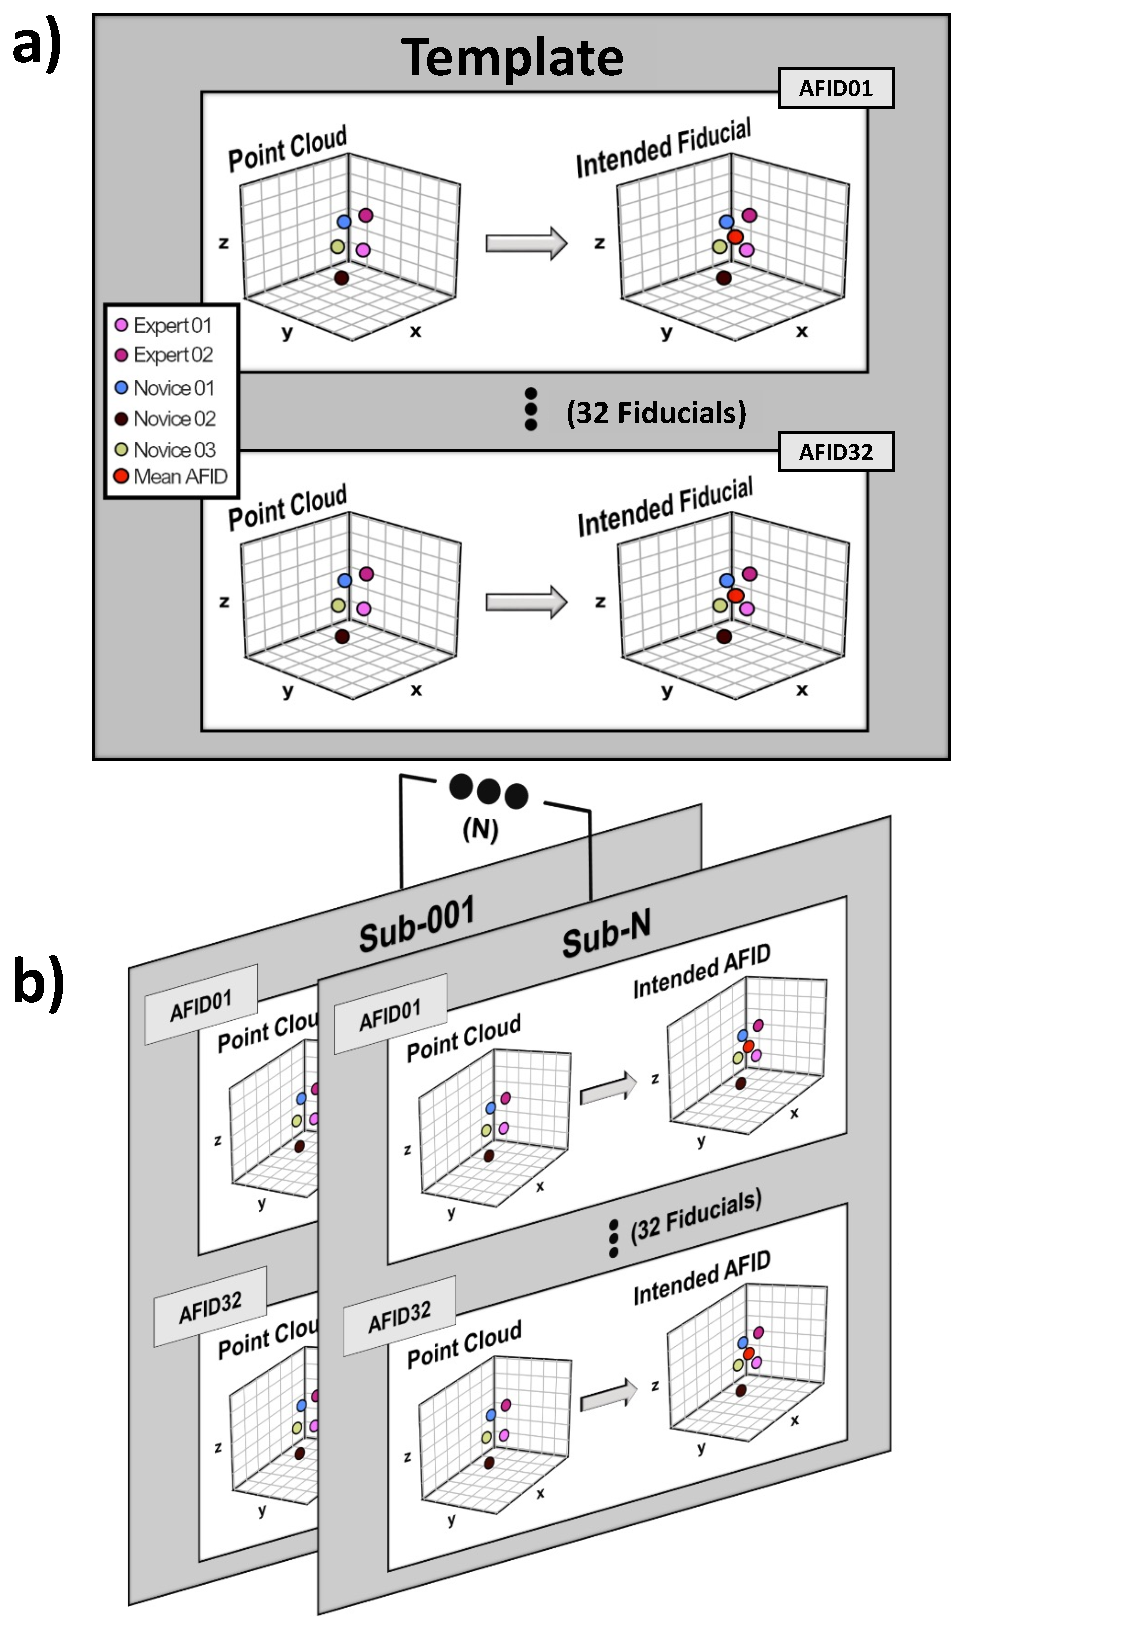
\includegraphics[width=1\linewidth]{figs/ch2_Figure_GT.pdf}
    \caption{Ground truth anatomical fiducial (AFID) placement on templates and datasets. (a,b) show the process of computing the intended AFID placement on a neuroimaging template or dataset, respectively. It is the mean of the rater point cloud at each AFID, referred to as “ground truth” in the text.}
    \label{fig:ch2_Figure_GT}
\end{figure}

To compute the mean AFLE, Euclidean distances from the ground truth fiducial location to each of the individual rater placements were averaged for each fiducial. The result is termed the subject or template mean AFLE per fiducial. This process was independently repeated for all subjects. All subject mean AFLEs were averaged to obtain a dataset mean AFLE per fiducial, as shown in Figure~\ref{fig:ch2_Figure_AFLE}a. Finally, the dataset mean AFLE per fiducial was averaged across all fiducials to yield the global dataset mean AFLE. 

In a similar fashion, global inter-rater AFLE was computed by measuring the pairwise Euclidean distance between all rater placements for each fiducial within a subject, averaging across fiducials to obtain a subject-level inter-rater AFLE, and then averaging across all subjects to produce the global dataset inter-rater AFLE (Figure~\ref{fig:ch2_Figure_AFLE}b).

\section{Data Records}

In total, we release the curated AFID placements and associated imaging of six datasets and fourteen openly available human brain templates—a total of more than 20,000 manually placed anatomical landmarks, representing more than 300 hours of human rater annotation.

All datasets have been deposited at DOI-issuing repositories such as Zenodo and OpenNeuro \cite{Taha2023-lt, Lau2023-db, Lau2023-op, Abbass2023-yl}, and conform to the Brain Imaging Data Structure (BIDS) directory hierarchy. Each dataset’s main directory contains (1) files about licensing and metadata, (2) imaging data directories organized per subject, and (3) a \texttt{derivatives} directory which includes AFID coordinates also organized per subject. We release both imaging and AFID annotation data. However, since some of the imaging datasets are protected under Data Usage Agreements (DUAs), the user needs to view and accept terms under DUAs before download.

For ease of acquiring the data, we merge released datasets and templates in a “super” dataset (\url{https://github.com/afids/afids-data}) which serves as a centralized repository for this data descriptor and can be used to install all of the imaging and AFID annotation data we release. In brief, the centralized repository (i.e., super dataset) has three main directories: (1) \texttt{data} — raw and curated coordinate files for datasets and templates alongside the MRI scans on which coordinates have been applied in BIDS format; (2) \texttt{notebooks} — code used for data curation and quality control; and (3) \texttt{other} — rater demographics, interactive glass brain showing applied coordinates, and a list of our curated brain landmarks.

Raw rater annotations were also released. These files have a \texttt{rater} label under the \texttt{desc} BIDS entity with session also encoded (if applicable). Additionally, curated mean placements (have a \texttt{groundtruth} tag in the \texttt{desc} BIDS entity) are made available. We make individual rater placements available so users have the opportunity to select the subset of rater placements for their intended application. However, we believe that our “ground truth” placements provide the best estimate as to where the true AFIDs are located.

The AFIDs coordinates are described using the Markups comma-separated values file (i.e., \texttt{*.fcsv}), which is generated after the raters save their placements on 3DSlicer. The \texttt{.fcsv} file contains coordinate data organized in rows for each of the 32 landmarks of interest, with columns describing the AFID and corresponding \texttt{x}, \texttt{y}, and \texttt{z} coordinates in native subject or template space. As for the imaging data, all dataset images used for annotations were BIDS compatible and made available in a compressed \texttt{NIfTI-1} format (i.e., \texttt{*.nii.gz}).

All AFID annotations generated in this study are publicly released under the terms of the Creative Commons Attribution 4.0 International (CC BY 4.0) license. This allows for unrestricted use, distribution, and adaptation of the AFID coordinates, provided appropriate credit is given to the original authors. In contrast, the neuroimaging data used to generate these annotations are subject to data use agreements (DUAs) specific to each source dataset. These agreements govern the redistribution and reuse of raw imaging data and must be reviewed and accepted by downstream users. To facilitate compliance, we provide a summary of the relevant DUAs in the \texttt{IMAGING\_DATA\_USE\_AGREEMENT.txt} file included with the repository.


\section{Technical Validation}
As detailed in the Methods section, all raters followed the standardized AFID protocol using publicly available documentation and training materials hosted at: \url{https://afids.github.io/afids-protocol}. To ensure that the fiducial placements released in this work are both accurate and reproducible, we assessed inter-rater and mean AFLE across all annotated datasets and templates. These metrics serve as a quality benchmark and reflect agreement between raters and their computed consensus ground truth. As summarized in Table~\ref{tab:afle_metrics}, placements were generally consistent within 1–2\,mm. Across all performances of the protocol, the global inter-rater AFLE was $1.73 \pm 0.34$\,mm, and the global mean AFLE was $0.99 \pm 0.32$\,mm.

\begin{table}[hbt!]
\centering
\caption{Summary of mean and inter-rater anatomical fiducial localization error (AFLE) metrics across all templates and datasets. Euclidean distances (ED) utilized shows how many distances were used in the validator process. Values are reported as mean ± standard deviation.}
\renewcommand{\arraystretch}{1.2}
\small
\begin{tabular}{
  >{\centering\arraybackslash}p{4cm}
  >{\centering\arraybackslash}p{6.1cm}
  >{\centering\arraybackslash}p{2cm}
  >{\centering\arraybackslash}p{2.5cm}
}
\toprule
\textbf{Template or Dataset} & \textbf{EDs utilized} & \textbf{Mean} & \textbf{Inter-rater} \\
\midrule
MNI152NLin2009bAsym  & Mean: 1,024; Inter-rater: 896 & 0.99 ± 1.11 & 1.07 ± 0.46 \\
MNIColin27           & Mean: 1,024; Inter-rater: 896 & 1.71 ± 2.78 & 1.36 ± 0.88 \\
Agile12v2016         & Mean: 1,024; Inter-rater: 896 & 1.10 ± 1.59 & 1.14 ± 0.48 \\
BigBrainSym          & Mean: 64; Inter-rater: 32     & 0.63 ± 0.50 & 1.25 ± 1.02 \\
MNI152NLin2009bSym   & Mean: 64; Inter-rater: 32     & 0.55 ± 0.26 & 1.09 ± 0.52 \\
PD-25                & Mean: 64; Inter-rater: 32     & 0.42 ± 0.24 & 0.83 ± 0.47 \\
MNI152Lin            & Mean: 128; Inter-rater: 192   & 1.07 ± 0.45 & 1.74 ± 0.74 \\
MNI152NLin2009cAsym  & Mean: 128; Inter-rater: 192   & 1.03 ± 0.40 & 1.67 ± 0.63 \\
MNI152NLin2009cSym   & Mean: 128; Inter-rater: 192   & 1.06 ± 0.47 & 1.67 ± 0.63 \\
MNI152NLin6Asym      & Mean: 128; Inter-rater: 192   & 1.16 ± 0.51 & 1.90 ± 0.86 \\
MNI152NLin6Sym       & Mean: 128; Inter-rater: 192   & 1.08 ± 0.54 & 1.73 ± 0.84 \\
MNI305               & Mean: 128; Inter-rater: 192   & 1.14 ± 0.41 & 1.85 ± 0.52 \\
OASIS30ANTs          & Mean: 128; Inter-rater: 192   & 0.78 ± 0.33 & 1.25 ± 0.51 \\
fsaverage            & Mean: 128; Inter-rater: 192   & 1.00 ± 0.44 & 1.65 ± 0.73 \\
AFIDs-HCP30          & Mean: 2,880; Inter-rater: 2,880  & 0.66 ± 0.22 & 1.15 ± 0.70 \\
AFIDs-OASIS30        & Mean: 2,880; Inter-rater: 2,880  & 0.94 ± 0.73 & 1.58 ± 1.02 \\
AFIDs-ADNI10         & Mean: 640; Inter-rater: 320  & 0.78 ± 0.90 & 1.55 ± 1.78 \\
LHSCPD               & Mean: 8,000; Inter-rater: 16,000 & 1.57 ± 1.16 & 2.01 ± 1.49 \\
SNSX                 & Mean: 5,952; Inter-rater: 5,952  & 0.96 ± 0.33 & 1.64 ± 1.37 \\
3T7T                 & Mean: 1,920; Inter-rater: 1,920  & 1.04 ± 0.83 &  1.74 ± 1.39  \\
\midrule
\textbf{Total or Average} & \textbf{Mean: }23,872; \textbf{Inter-rater:} 32,160 & \textbf{1.14 ± 0.36} & \textbf{1.73 ± 0.34} \\
\bottomrule
\end{tabular}
\label{tab:afle_metrics}
\end{table}

To highlight a central use case of our released data in the context of image registration, we employed \texttt{fMRIPrep} (v21.0.1; \cite{Esteban2019-oz}) which is a commonly used neuroimaging software to analyze MRI data. \texttt{fMRIPrep} leverages ANTs \cite{Avants2008-ek} to perform deformable registration to a stereotactic space. The pipeline was run with default settings on all T1w MRI scans. Below, we examined the consensus AFRE associated with \texttt{fMRIPrep} at multiple levels of granularity (Figure \ref{fig:ch2_Figure_afres}).

\begin{figure}[hbt!]
    \centering
    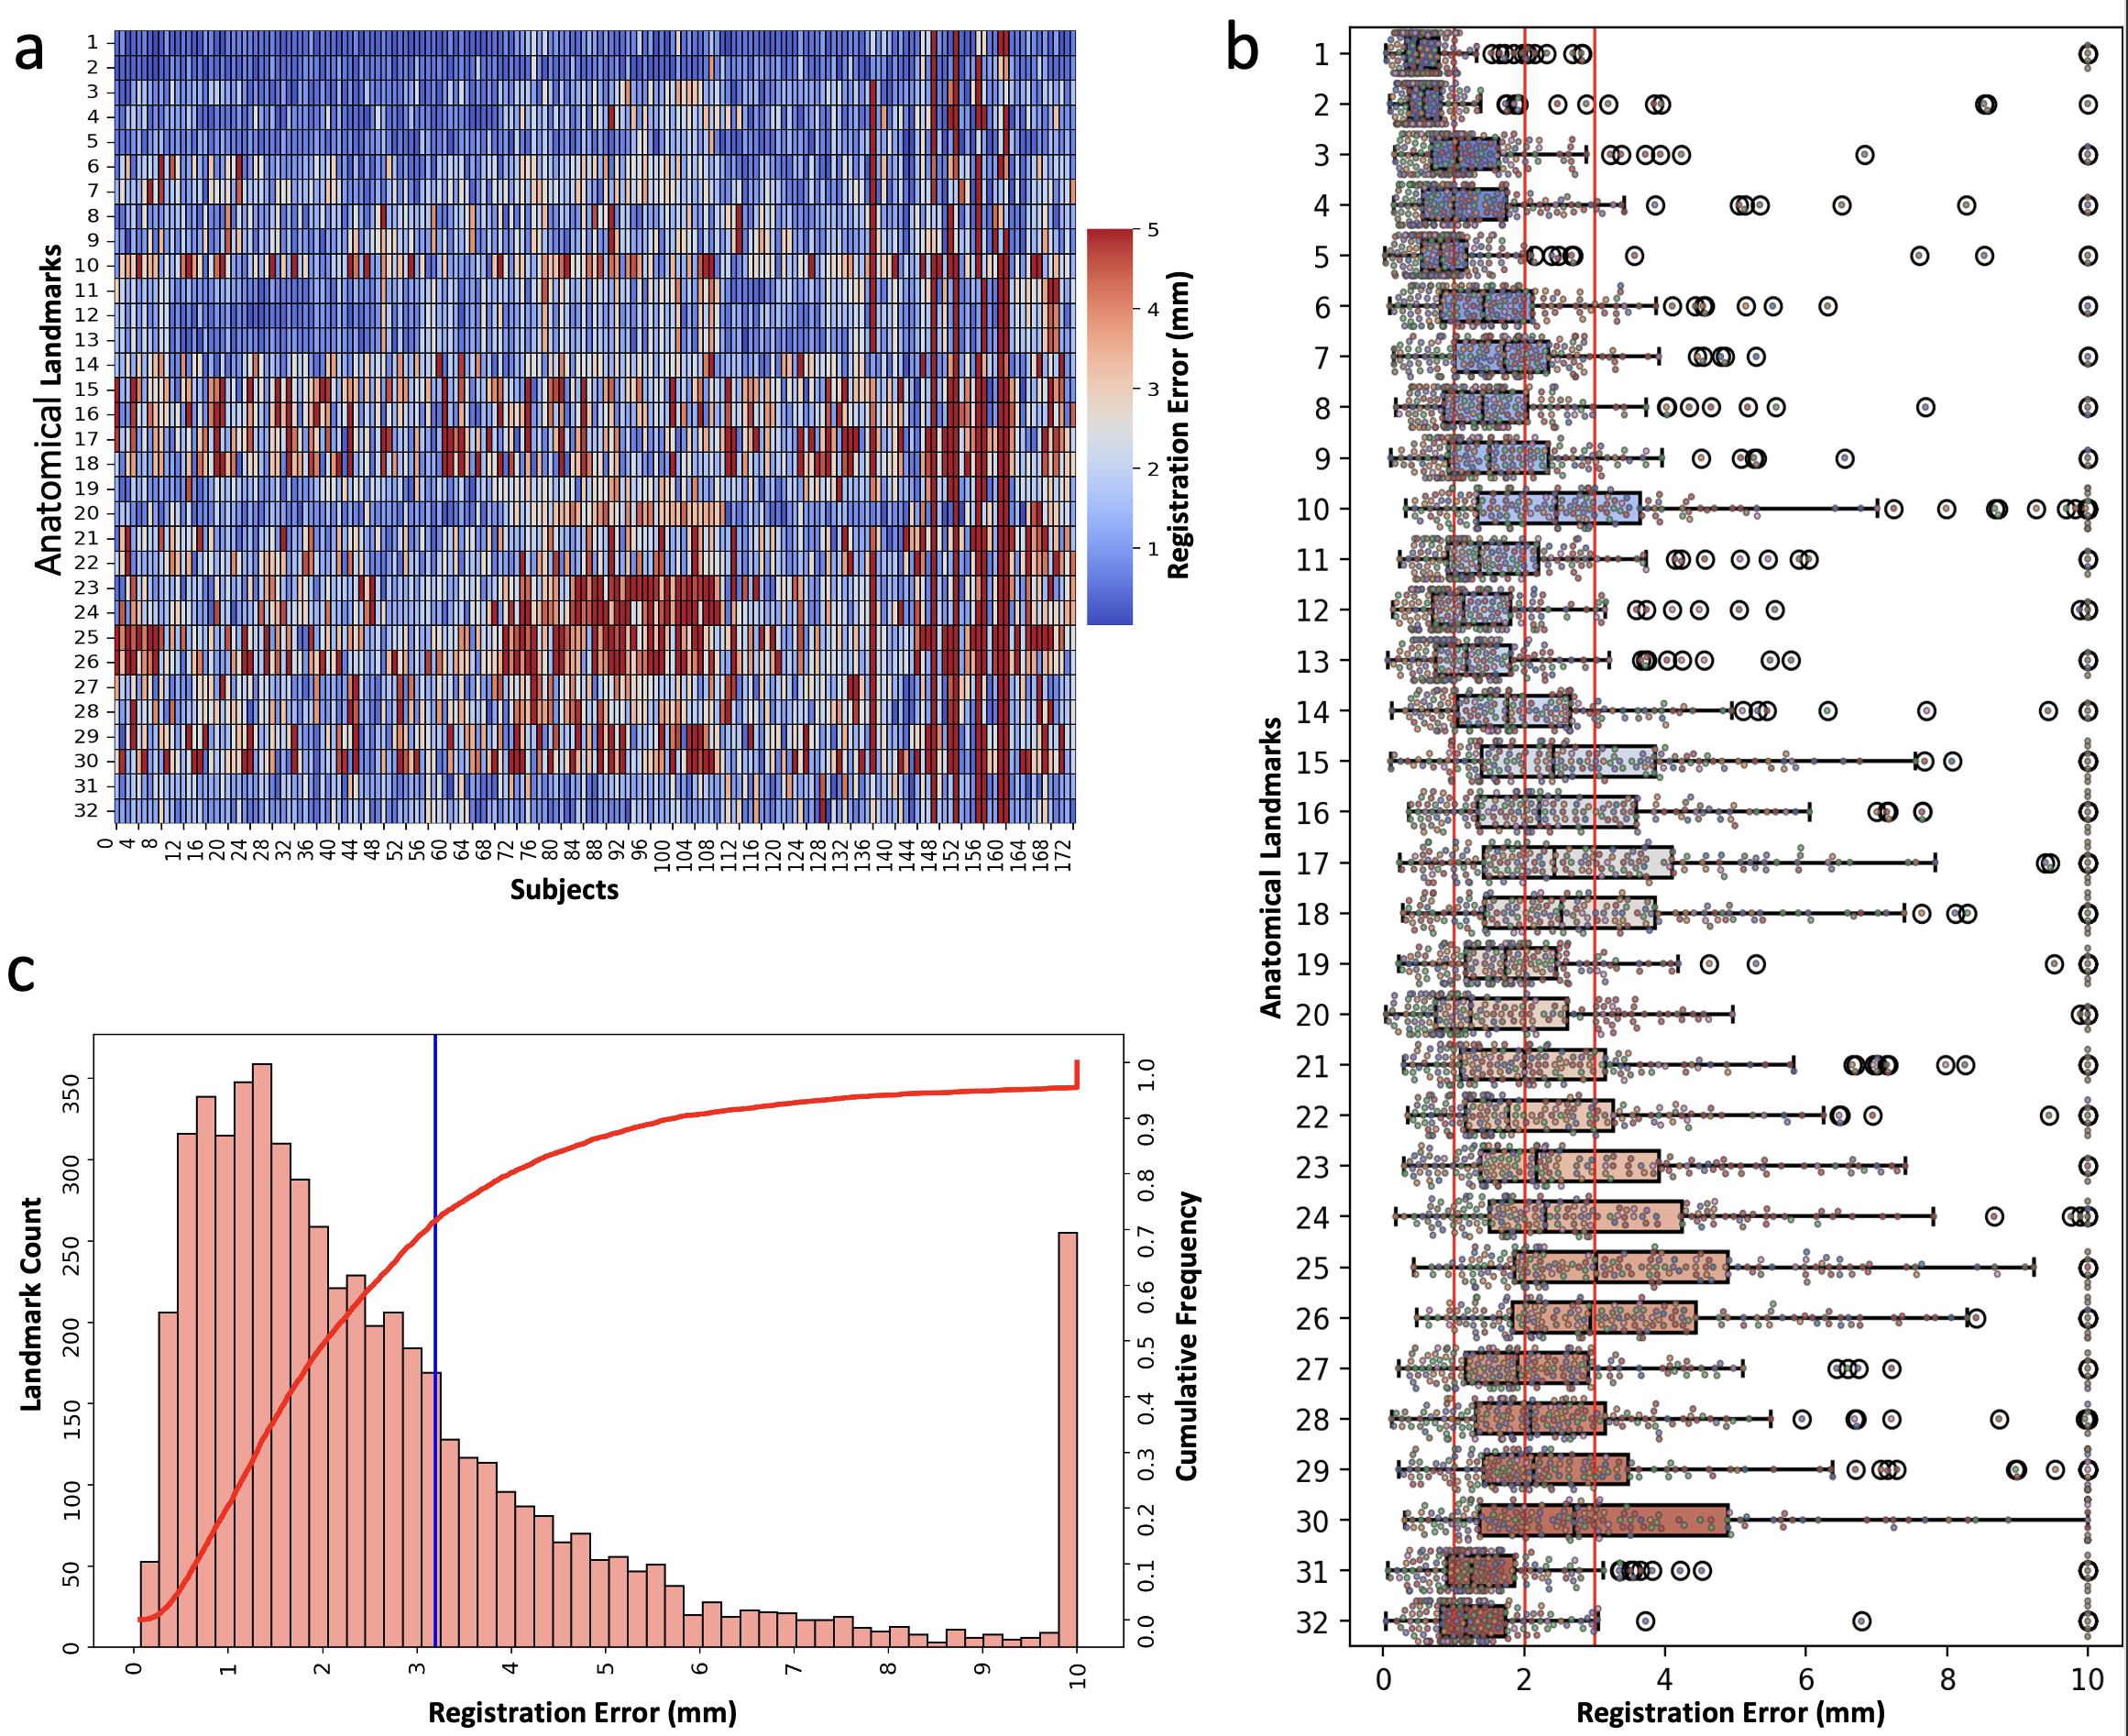
\includegraphics[width=1\linewidth]{figs/ch2_Figure_AFREs.png}
    \caption{Multi-level analysis of anatomical fiducial registration error (AFRE). (a) Heatmap of registration error across 173 subjects and 32 anatomical landmarks (AFIDs). Each cell reflects the Euclidean distance between a registered and reference landmark. Warmer colors indicate higher error, with lateral and inferior structures exhibiting greater variability. (b) Distribution of AFRE for each AFID using boxplots. Red vertical lines indicate 1\,mm, 2\,mm, and 3\,mm thresholds. Most midline and brainstem landmarks (AFIDs 1-5) show \(<\)2 mm error, while ventricular horns and occipital structures (AFIDs 15-18 and 21-26) exhibit broader error distributions with frequent outliers. (c) Histogram and cumulative frequency plot of AFREs across the full dataset (5,536 AFIDs). The red curve traces cumulative frequency and the blue line represents the mean AFRE across the full dataset which was 3.19~\(\pm\)~4.01. Global Median AFRE \(\pm\) interquartile range was: 2.02~\(\pm\)~2.35~mm.
    }
    \label{fig:ch2_Figure_afres}
\end{figure}

At the subject level, AFREs form a matrix with rows representing AFIDs and columns representing subjects (Figure~\ref{fig:ch2_Figure_afres}a). This heatmap highlights both regional and subject-specific outliers. In our cohort, lateral and inferior temporal horn AFIDs (21–26) consistently showed higher AFREs, whereas midline structures such as the AC and PC (AFIDs 1 and 2) exhibited lower and more stable AFREs. AFID-wide summaries across subjects reveal broader trends (Figure~\ref{fig:ch2_Figure_afres}b). Midline and brainstem AFIDs (1-9) generally had \(<\)2 mm median AFREs with tight distributions, while lateral and ventricular AFIDs (15-18)—including the temporal (21-26) and occipital (29, 30) horns—showed wider variability and frequent outliers exceeding 5\,mm, consistent with greater anatomical variability in those regions. At the dataset level (Figure~\ref{fig:ch2_Figure_afres}c), a histogram and cumulative frequency plot of 5,536 AFREs revealed a mean error of 3.19\(\pm4.01\), with an interquartile range (IQR) of 1.14–3.49\,mm. While half of the AFREs fell below the commonly accepted 2\,mm threshold for stereotactic applications, a substantial proportion exceeded this benchmark—indicating that even within well-curated neuroimaging pipelines, registration inaccuracy must undergo quantitative review. In particular, the upper quartile of values approached or exceeded 3.5\,mm, which may impact downstream localization tasks that depend on precise spatial correspondence. These findings underscore the need to move toward quantitative (i.e., millimetric), region- and subject-specific quality assessments to detect and mitigate subtle registration failures. 

To investigate registration error across datasets (Figure~\ref{fig:ch2_Figure_bias}a), we performed principal component analysis (PCA) on directional AFREs (Figure~\ref{fig:ch2_Figure_bias}b). Each subject’s error profile was represented as a 3D vector per AFID, capturing spatial misalignment after nonlinear registration. We visualized these profiles in PCA space and computed silhouette scores using scanner type as the class label: 1.5T (GAD+), 3T, and 7T. A high silhouette score in this context reflects scanner-dependent structure in the AFRE space—indicating that the imaging modality systematically shapes misalignment patterns. This is undesirable when contextualized with a high global AFRE, as it suggests bias introduced by acquisition or preprocessing rather than true anatomical variance.

Among modalities, the 7T group demonstrated the best global AFRE (median \(\pm\) IQR: 1.78~\(\pm\)~0.77 mm), followed by the 3T group (1.82~\(\pm\)~0.53 mm), with the 1.5T(GAD+) group performing worst (2.39~\(\pm\)~0.39~mm). However, 1.5T(GAD+) group showed the highest silhouette score (0.303), indicating strong dataset-specific clustering of errors. Meanwhile, the silhouette scores for the 3T and 7T groups were 0.175 and 0.213, respectively. These findings must be considered in light of template contrast. All scans were registered to the MNI152NLin2009bAsym template, which likely favored alignment of non-contrast images while introducing more dataset specific AFRE profiles in 1.5T(GAD+) and 7T group perhaps due mismatch in contrast. An important limitation of our dataset is its heterogeneity: both 1.5T and 7T groups included Parkinson’s disease (PD) patients, while 3T scans were limited to healthy controls and subjects with atypical anatomy. As such, these findings should definitely not be interpreted as purely scanner- and acquisition-driven. Rather, this analysis serves as a proof-of-concept illustrating that registration bias can emerge from scanner characteristics, cohort composition, and template choice. A more definitive and targeted assessment would require paired datasets across modalities (e.g., test-retest data) to disentangle modality effects from subject-specific anatomy. Taken together, these results highlight that scanner characteristics, template selection, and cohort brain morphology jointly influence registration performance. For high-precision applications like deep brain stimulation (DBS), where analysis is conducted in stereotactic space, contrast harmonization and millimetric accuracy are critical, as registration errors can approach the size of functional targets themselves \cite{Hollunder2024-wc}.

\begin{figure}
    \centering
    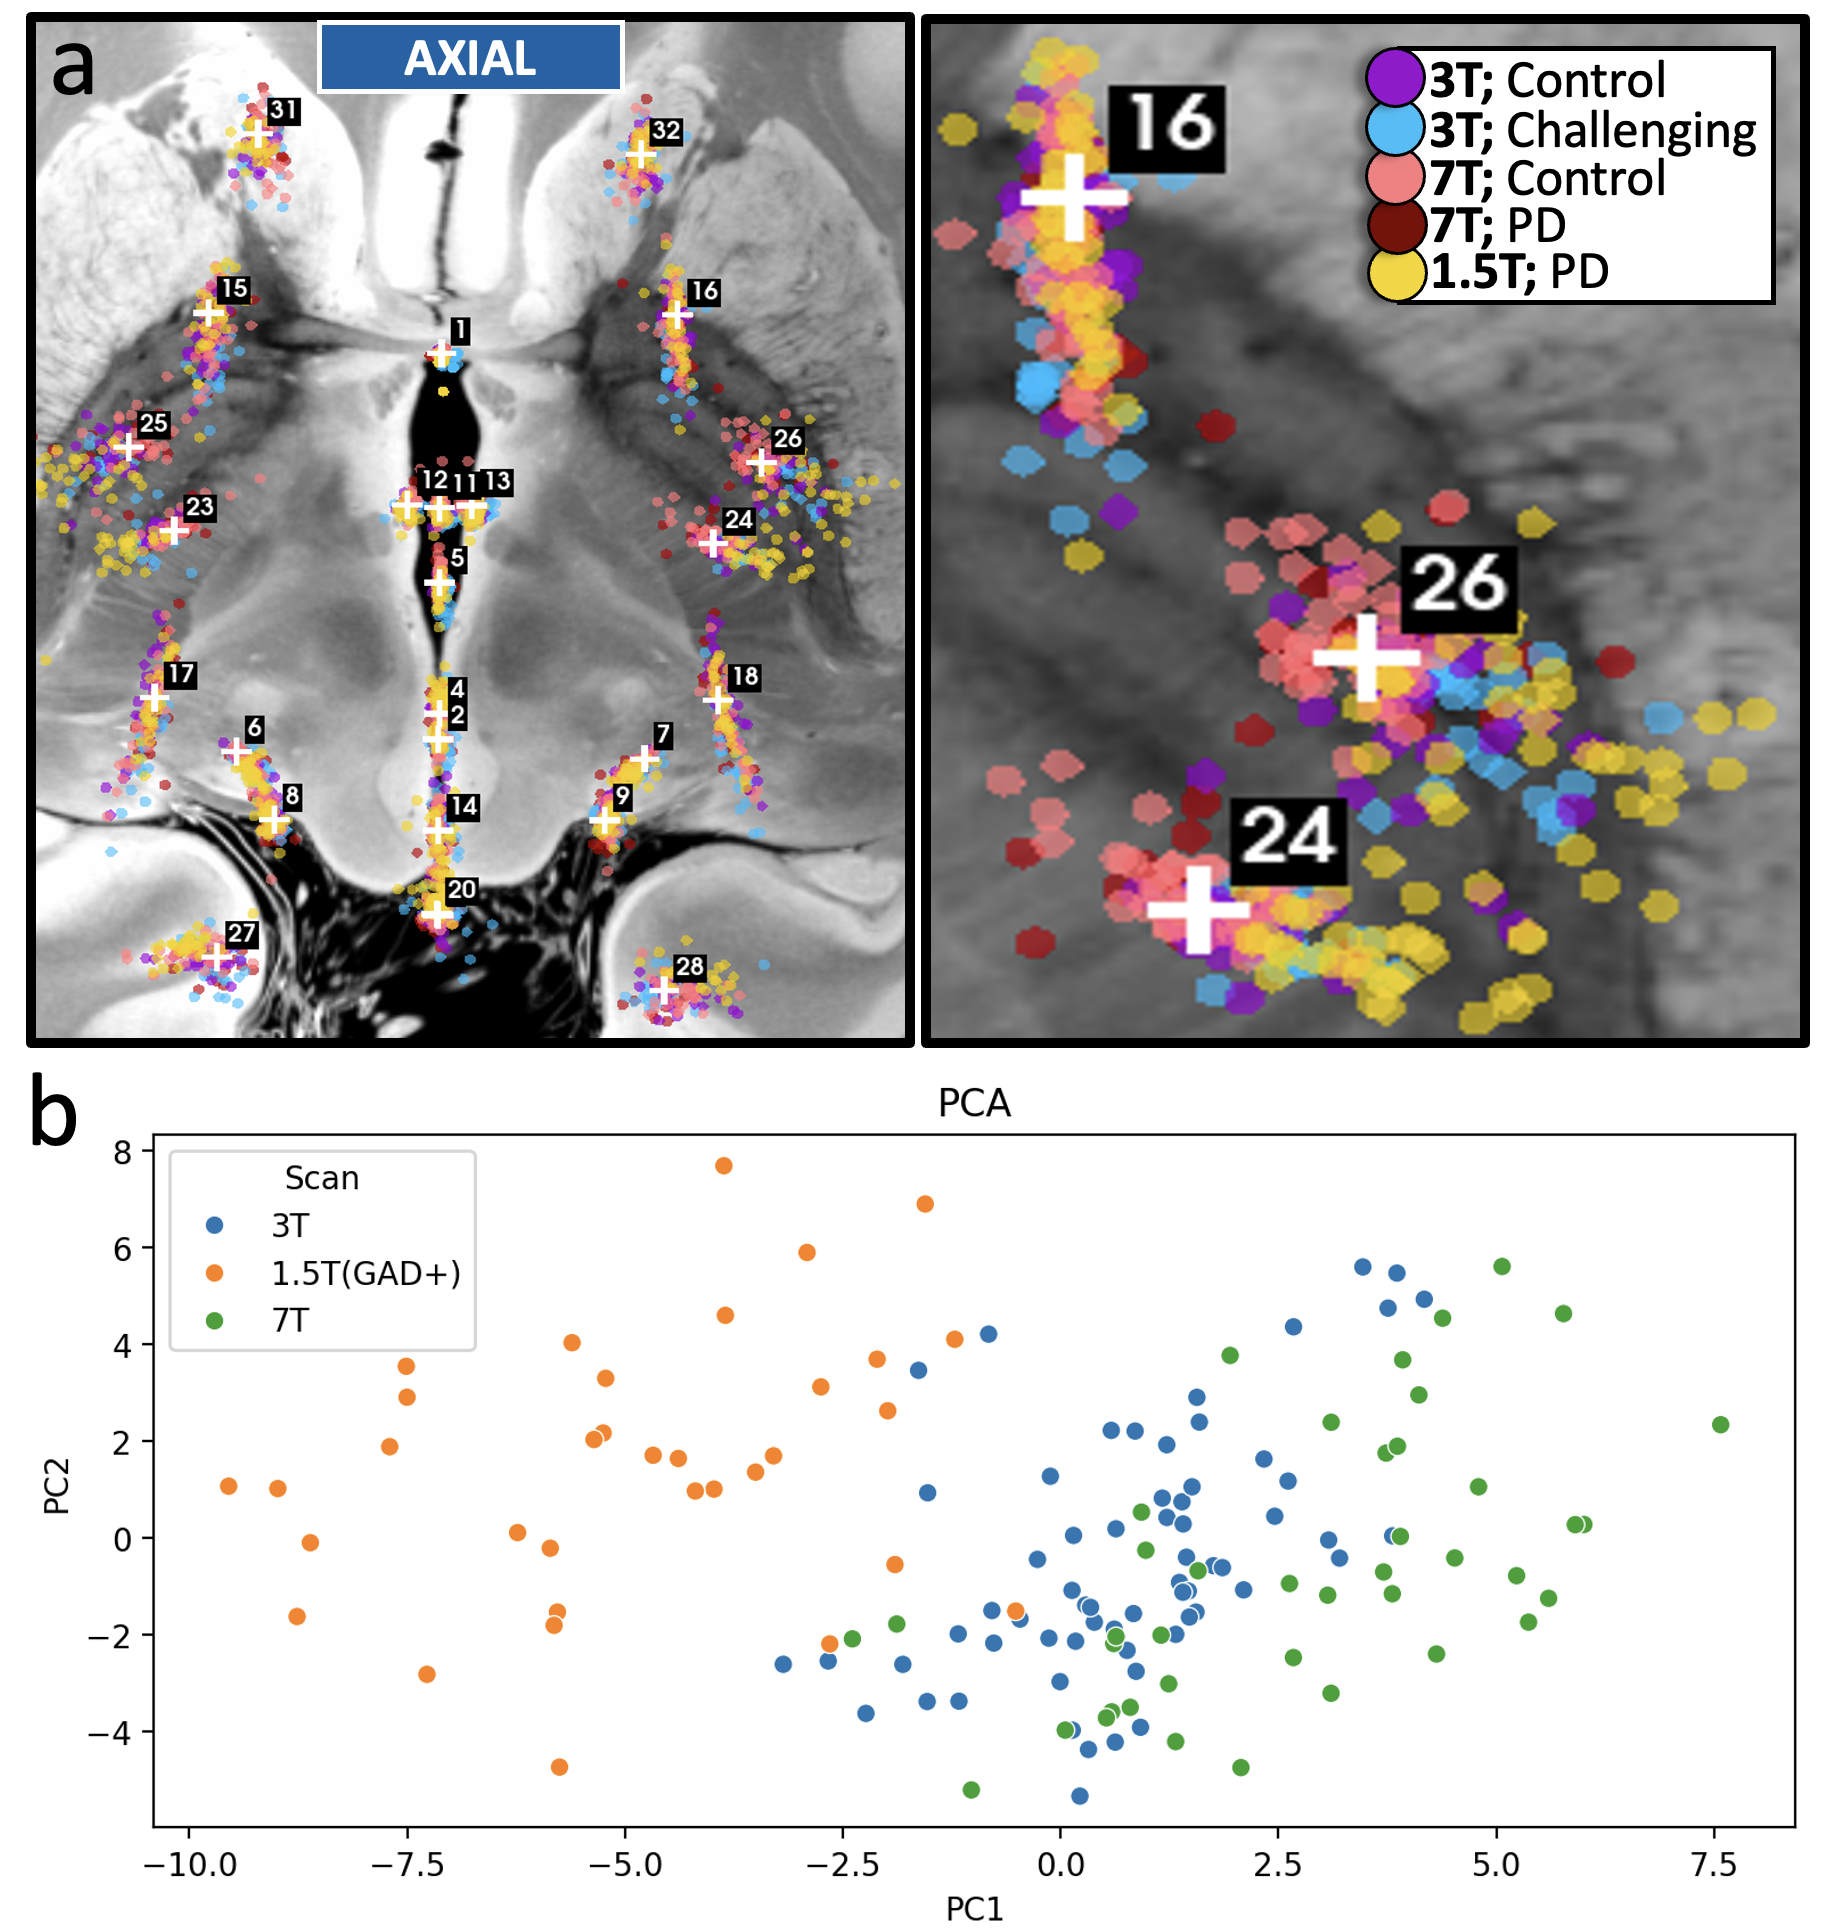
\includegraphics[width=1\linewidth]{figs/ch2_Figure_bias.png}
    \caption{Biases and clustering of anatomical fiducial registration error (AFRE) across datasets. (a) Axial view showing AFRE across subjects in stereotactic space, with zoomed-in view of AFIDs 16, 24, and 26. Each colored dot represents the registered location of an AFID for a subject; white crosses indicate the ground truth location. Points are color-coded by dataset and scan type. (b) Dimensionality reduction of AFRE profiles using principal component analysis (PCA) reveals contrast-dependent clustering. Each point represents a subject's AFRE profile across all AFIDs, colored by MRI group. Notably, 1.5T(GAD+) scans (orange) form a distinct cluster seperate from 3T (blue) and 7T scans (green), suggesting modality-driven variance in registration outcomes. These findings highlight a qualitative bias introduced during registration, with potential implications for pooled multi-site analyses in stereotactic space.
    }
    \label{fig:ch2_Figure_bias}
\end{figure}



\section{Usage Notes and Data Access}
We recommend loading the shared AFID annotation files (\texttt{*.fcsv}) in 3D Slicer alongside their associated imaging data, all of which are organized in BIDS format to facilitate intuitive navigation. The local neuroimaging datasets released in this work—specifically, LHSCPD and SNSX—will continue to undergo quality control and will be expanded as additional participants are recruited. Future versions of this data descriptor may include new anatomical landmarks, provided they meet validation criteria established in prior studies.

Access to imaging data is granted once users accept the respective Data Usage Agreements (DUAs). Instructions for gaining access are provided with each dataset. For the \textbf{AFIDs-HCP} dataset, users must register for an account at the HCP portal (\url{https://db.humanconnectome.org}) and accept the DUA to receive an access key for use when cloning the repository. For the \textbf{AFIDs-OASIS} dataset, users must accept the DUA at \url{https://www.oasis-brains.org}, though no credentials are required for access. Permission to redistribute HCP and OASIS imaging data has been obtained. The locally generated \textbf{SNSX} and \textbf{LHSCPD} datasets are shared under a Creative Commons license, and thus no further action is required.

All datasets used in this study can be downloaded using DataLad (\cite{Halchenko2021-px}; \url{https://www.datalad.org/#install}, following acceptance of any required DUAs. After installing DataLad, users may retrieve the full collection with the following commands:
\begin{minted}[fontsize=\small, bgcolor=bg, linenos, breaklines]{yaml}
datalad install -r https://github.com/afids/afids-data.git
cd afids-data
datalad get -r .
\end{minted}

Alternatively, users may choose to retrieve specific datasets or subsets by navigating to the desired subdirectory within the installed dataset and calling:
\begin{minted}[fontsize=\small, bgcolor=bg, linenos, breaklines]{yaml}
datalad get -r .
\end{minted}

If DUA acceptance is required, the system will prompt users to enter relevant credentials before download. Additional information on accessing specific datasets and resolving download issues is available at our centralized repository. Although individual dataset repositories remain accessible, we strongly encourage users to download and work with the centralized dataset for consistency and ease of use. The code used for technical validation as well as prior AFID studies can be found on the GitHub repository page \url{https://github.com/afids}, including the validator tool \url{https://github.com/afids/afids-validator}.

\section{Conclusion}
In this work, we validated the AFIDs framework across a range of MRI field strengths, achieving a global mean AFLE of less than 1 mm. We also evaluated the global AFRE using a widely adopted neuroimaging pipeline and identified contrast-dependent registration bias related to MRI field strength. Importantly, we make all coordinate data publicly available to support downstream applications in image registration, automated landmark localization, and coordinate-based brain mapping.